Tritium is the only radioactive isotope of hydrogen present in the environment. Tritium was produced artificially for the first time in $1934$ in neutron capture on deuterium by Ernest Rutherford, Mark Oliphant and Paul Harteck \cite{TritiumDiscovery} and was isolated in 1939 by Luis Walter Alvarez and Robert Cornog \cite{TritiumIsolate}, who discovered that tritium is radioactive. Tritium has a half-life time of $T_{1/2}= 12.32$ years. It decays exclusively through $\beta$ radiation to the ground state of the $\ce{^{3}_{2}He}$ isotope of helium, which is a stable nuclei, through the process,

\begin{equation}
\ce{^{3}_{1}H} \longrightarrow \ce{^{3}_{2}He}  + \ce{e^-}  + \ce{\overline{\nu}_e}
\label{eq:TritiumDecay}
\end{equation}
In Figure \ref{fig:TritiumDecay}, the scheme of tritium energy levels is shown. In this decay it is not possible to detect the neutrino because of its extremely weak interaction with matter ($\sigma \approx 10^{-44} ~ \cm^2$) \cite{CrossSeccionNeutrino} and, since $\ce{^{3}He}$ has a much larger mass than electrons and neutrinos, the energy carried by the daughter nucleus is very small. Therefore, the detection of tritium is done through its decay electron. 

\begin{figure}
\centering
    \begin{subfigure}[b]{0.55\textwidth}
    \centering
    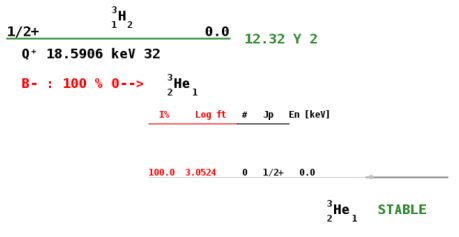
\includegraphics[width=\textwidth]{2Introduction/esquema_niveles_energeticos.png}  
    \caption{\label{subfig:Energy_levels}}
    \end{subfigure}
    \hfill
    \begin{subfigure}[b]{0.4\textwidth}
    \centering
    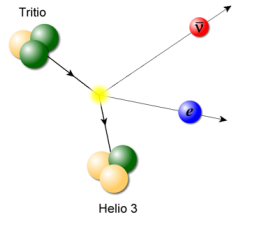
\includegraphics[width=\textwidth]{2Introduction/representacion_desintegracion.png}  
    \caption{\label{subfig:GraphicDesintegration}}
    \end{subfigure}
 \caption{a) Tritium energy levels \cite{TritiumDecayEnergyLevels}. b) Graphical representation of tritium decay \cite{TritiumDecayImage}.}
 \label{fig:TritiumDecay}
\end{figure}

The energy released in the tritium decay is $Q_\beta=18.6~\keV$, shared between the decay products. Therefore, the energy spectrum of the decay electrons is a continuum with a maximum value of $18.6~\keV$, as shown in Figure \ref{fig:TritiumDecaySpectrum}. This energy spectrum has an average of $5.7~\keV$ and the most likely energy is around $4.5~\keV$. Tritium is the radioactive isotope with the lowest energy released in $\beta$ decay \cite{TritiumHandling}. Consequently, the $\beta$ particle emitted has a very short mean free path, given in Table \ref{tab:MeanFreePathTritium}, which is a major issue in tritium detection, as the electron detection requires a highly sensitive detector. Tritium electrons have a low penetration in the human body and they are easily stopped by clothes or laboratory gloves, resulting in a low radiological hazard from external exposure. Nevertheless, the danger of tritium increases when it is ingested or inhaled since it binds to the molecules of the human body and undergoes the same chemical reactions as hydrogen.

\begin{figure}[h]
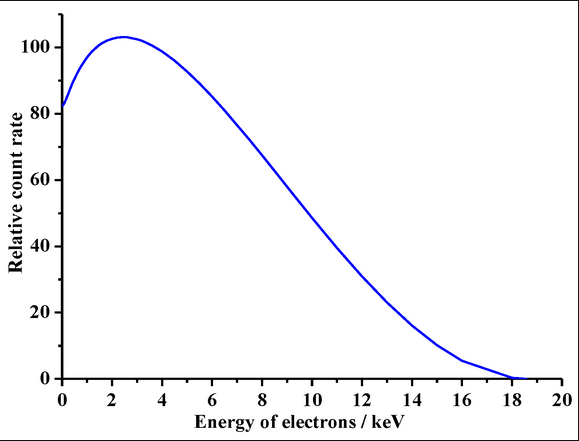
\includegraphics[scale=0.85]{2Introduction/Espectro_tritio.png}
\centering
\caption{Energy spectrum of tritium electrons ~\cite{TritiumEspectrum}.\label{fig:TritiumDecaySpectrum}}
\end{figure}

\begin{table}[h]
\centering{}%
\begin{tabular}{lcc}
\toprule 
Energy & $5.7~\keV$ & $18.6~\keV$ \tabularnewline
\midrule
Material & \multicolumn{2}{c}{Penetration Depth} \tabularnewline
\midrule
\midrule 
$\ce{\ce{^{3}_{1}H_2}}$ & 0.26 cm & 3.2 cm \tabularnewline
Air & 0.036 cm & 0.45 cm \tabularnewline
\parbox{10em}{ Water, soft tissue\\  (solid matter with a \\  density of $1~\gram\cdot\cm^{-3}$)} & 0.42 $\mu\meter$ & 5.2 $\mu\meter$ \tabularnewline
\bottomrule
\end{tabular}
\caption{Penetration depth of decay electrons of mean ($5.7~\keV$) and maximum ($18.6~\keV$) energies in different media (tritium gas, air at STP and water)~\cite{MeanFreePathDocument}.}
\label{tab:MeanFreePathTritium}
\end{table} 

Tritium is naturally produced in the environment through the interaction of cosmic rays with elements of the upper atmosphere like nitrogen $\ce{^{14}N}(\ce{n},\ce{^{3}H})\ce{^{12}C}$ \cite{TritiumHandling} and oxigen $\ce{^{16}O}(\ce{n},\ce{^{3}H})\ce{^{14}N}$ \cite{OxigenTritium}. Around 99\% of cosmogenic tritium forms water (\ce{HTO}) and reaches the Earth's surface as rain with an estimated production rate of $4\cdot 10^6 ~\curie/$yr ($1.48 \cdot 10^8 ~\giga\becquerel/$yr), producing a tritium concentration of $0.6-1.2~\becquerel/\liter$ in precipitation \cite{CommonEmissionTritium, TritiumHandling}. 

Tritium can be produced artificially in the environment from different anthropogenic sources \cite{CommonEmissionTritium, TritiumHandling}. There is a large amount of tritium which was produced in military nuclear explosions between 1945 and 1975, with an estimated total production of $8 \cdot 10^9~\curie$ ($2.96 \cdot 10^{11}~\giga\becquerel$), a part of which remains to the date. In these nuclear explosions, tritium was produced mainly from the nuclear reactions $\ce{^{14}N}(\ce{n},\ce{^{3}H})\ce{^{12}C}$ and $\ce{^{2}H}(\ce{n},\gamma)\ce{^{3}H}$. Tritium is produced by commercial producers of radioluminiscent and neutron generator devices ($1 \cdot 10^6~\curie/$yr), nuclear power and defense industries (around $2 \cdot 10^6~\curie/$yr) and several research facilities and nuclear reactors for energy production ($2 \cdot 10^6~\curie/\giga\watt$yr). The production cross sections of the relevant processes are shown in Table \ref{tab:NuclearReactionsTritiumProduction}.

\begin{table}[htbp]
\centering{}%
\begin{tabular}{lccc}
\toprule 
Source & Origin & Nuclear reaction & Cross section ($\barn$)\tabularnewline
\midrule
\midrule 
$\ce{^{2}_{1}H}$ & Water coolant & $\ce{^{2}_{1}H}(\ce{n},\gamma)\ce{^{3}_{1}H}$ & $5.2 \cdot{} 10^{-4}$ \tabularnewline
$\ce{^{3}_{2}He}$ & Helium coolant & $\ce{^{3}_{2}He}(\ce{n},\ce{p})\ce{^{3}_{1}H}$ & $5330$ \tabularnewline
\vspace{0.1cm}$\ce{^{6}_{3}Li}$ & Moderator & $\ce{^{6}_{3}Li}(\ce{n},\alpha)\ce{^{3}_{1}H}$ & $940$ \tabularnewline
$\ce{^{10}_{5}B}$ & \parbox{8em}{\centering Moderator,\\ control rods} & $\ce{^{10}_{5}B}(\ce{n},2\alpha)\ce{^{3}_{1}H}$ & $3835$ \tabularnewline 
\bottomrule
\end{tabular}
\caption{Most common nuclear reactions of artificial tritium production~\cite{CommonEmissionTritium}.}
\label{tab:NuclearReactionsTritiumProduction}
\end{table}

Tritium levels in water of the environment, excluding the current anthropogenic radioactive sources, are between $1$ and $4~\becquerel/\liter$, larger than expected from cosmogenic background levels ($0.6-1.2~\becquerel/\liter$) \cite{FranceTritiumEnvironment}. This excess is attributed to nuclear weapon tests. Tritium levels in rivers around a NPP are between $1$ and $10~\becquerel/\liter$ and even between $20$ and $50~\becquerel/\liter$ at the water discharge site of NPPs \cite{FranceTritiumEnvironment}, where the produced tritium is partially or totally released into the environment, mainly in $\ce{HTO}$ form.

The effect of NPPs on tritium levels in the environment can be observed in the REM data, for example for the case of the Cofrentes NPP. The tritium level is measured in three different places along the Júcar river, marked on the map shown in Figure \ref{fig:SamplingLocations}. P1 is located on the river $6~\kilo\meter$ upstream from the NPP, and P2 and P3 are located $1$ and $5~\kilo\meter$ downstream, respectively. The level of tritium measured in these three locations is shown as a function of time in Figures \ref{subfig:TritiumL6kB}, \ref{subfig:TritiumL1kA} and \ref{subfig:TritiumL5kA} respectively. In these figures, the detection limit and the measured activity are plotted with white and green dots, respectively. The measured activity is only displayed when it is larger than the corresponding detection limit. The tritium level in the river is larger near the discharge of the NPP and decreases $4~\kilo\meter$ downstream, as can be seen from these data. Two additional measurements of the tritium level in groundwater, points S1 and S2 on the map in Figure \ref{fig:SamplingLocations}, located $1~\kilo\meter$ upstream and downstream from the NPP, respectively, are included. Both tritium levels are shown in Figures \ref{subfig:TritiumLG1kB} and \ref{subfig:TritiumLG1kA}, respectively, where it can be observed that they are below the detection limit. It is important to note that, although environmental tritium level is affected by the NPP in the case of Cofrentes, these levels are below the maximum allowed limit. The maximum level of tritium measured since January 2, 2006 is around $32~\becquerel/\liter$, below the limit of $100~\becquerel/\liter$ recommended by the Euratom 2013 directive.

\begin{figure}[hbtp]
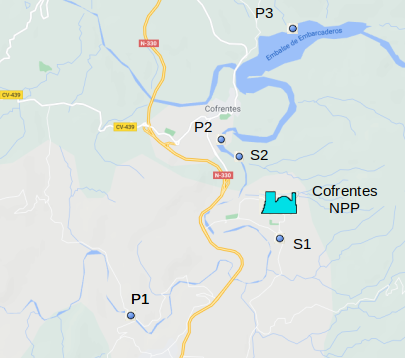
\includegraphics[scale=0.5]{2Introduction/CofrentesMaps.png}
\centering
\caption{Tritium sampling locations around Cofrentes NPP.\label{fig:SamplingLocations}}
\end{figure}

\begin{figure}
\centering
    \begin{subfigure}[b]{0.7\textwidth}
    \centering
    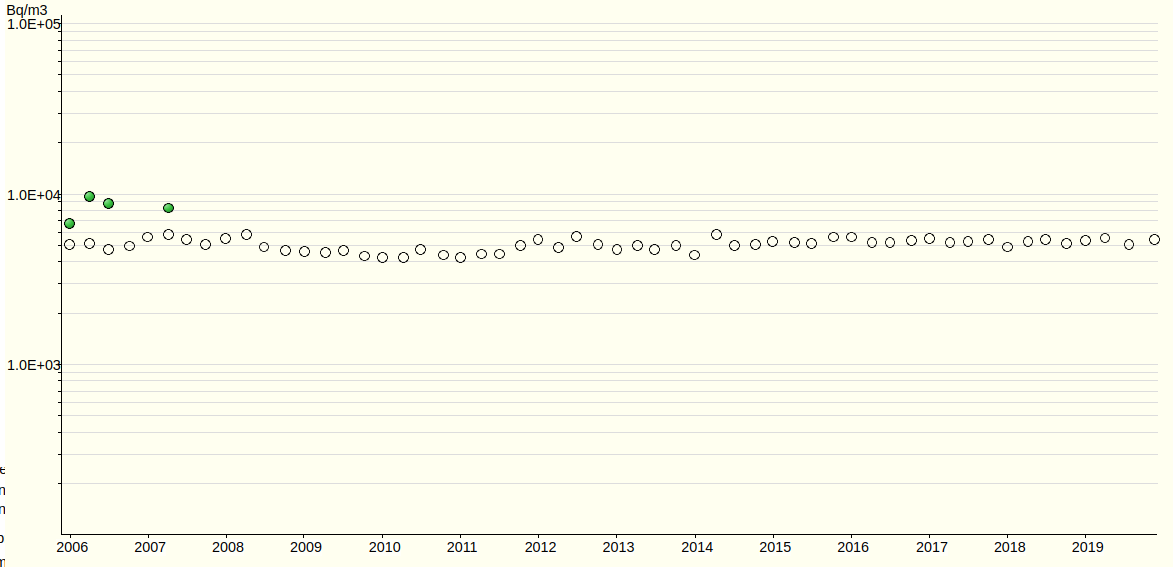
\includegraphics[width=\textwidth]{2Introduction/6km_before.png}  
    \caption{\label{subfig:TritiumL6kB}}
    \end{subfigure}
    \hfill
    \begin{subfigure}[b]{0.7\textwidth}
    \centering
    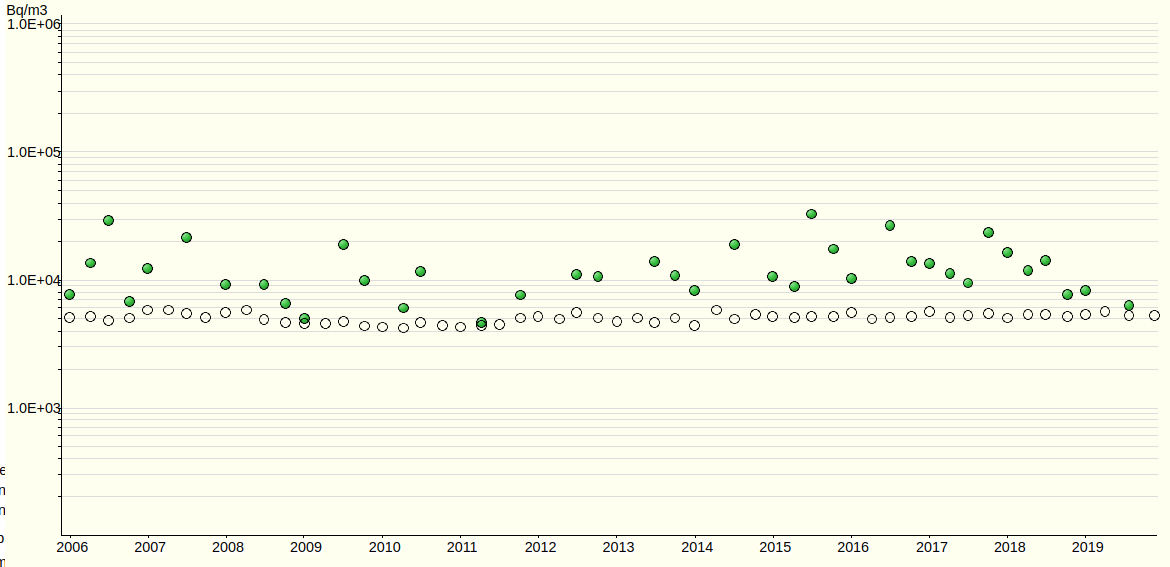
\includegraphics[width=\textwidth]{2Introduction/1km_after.png}  
    \caption{\label{subfig:TritiumL1kA}}
    \end{subfigure}
    \hfill
    \begin{subfigure}[b]{0.7\textwidth}
    \centering
    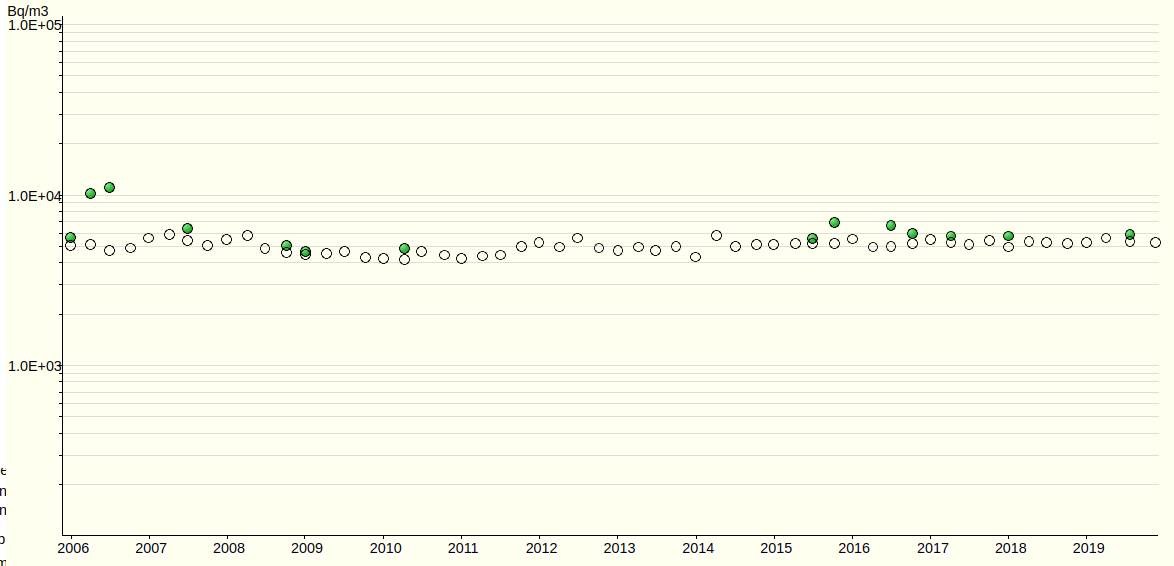
\includegraphics[width=\textwidth]{2Introduction/5km_after.png}  
    \caption{\label{subfig:TritiumL5kA}}
    \end{subfigure}
 \caption{Tritium activity levels in surface water around Cofrentes NPP from January $2006$ to November $2019$. a) $6~\kilo\meter$ upstream. b) $1~\kilo\meter$ downstream. c) $5~\kilo\meter$ downstream. The white points are the detection limits and the green points are the measured activity when this is above the detection limit~\cite{REM}. The maximum level of tritium measured since January 2, 2006 is around $32~\becquerel/\liter$.}
 \label{subfig:MeasurementsCofrentesSurface}
\end{figure}

\begin{figure}
\centering
    \begin{subfigure}[b]{0.7\textwidth}
    \centering
    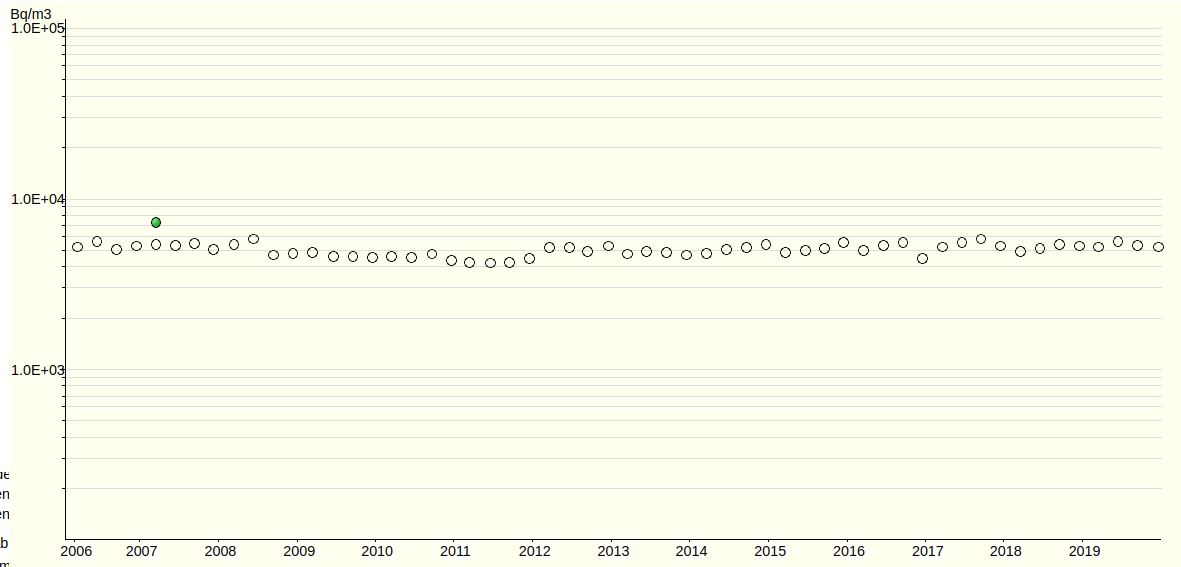
\includegraphics[width=\textwidth]{2Introduction/Subterranea_before.png}  
    \caption{\label{subfig:TritiumLG1kB}}
    \end{subfigure}
    \hfill
    \begin{subfigure}[b]{0.7\textwidth}
    \centering
    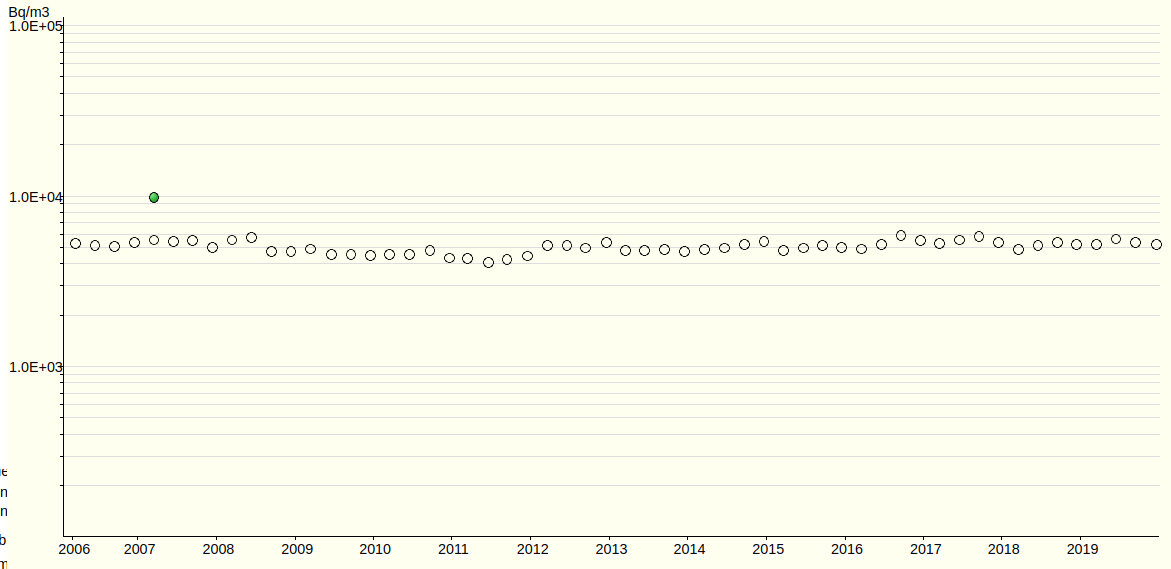
\includegraphics[width=\textwidth]{2Introduction/Subterranea_1_km_later.png}  
    \caption{\label{subfig:TritiumLG1kA}}
    \end{subfigure}
 \caption{Tritium activity levels in groundwater around Cofrentes NPP from January $2006$ to November $2019$~\cite{REM}. a) $1~\kilo\meter$ upstream from the NPP. b) $1~\kilo\meter$ downstream from the NPP.}
 \label{fig:MeasurementsCofrentesGroundWater}
\end{figure}

Tritium can be absorbed in our body by inhalation and ingestion. Tritium is present in three different chemical forms, gaseous tritium (mainly HT), tritiated water (mainly HTO) and organically bound tritium (OBT):

\begin{enumerate}
\item{} Gaseous tritium, usually found mixed in the air, is the least harmful form since less than a $(3-5) \cdot{} 10^{-3}~\%$ is absorbed by the human body, which is negligible \cite{TritiumHandling}. However, gaseous tritium can be transformed into tritiated water, more harmful from the radiological point of view \cite{TritiumHandling}, through oxidation and exchange reactions,

\begin{equation}
\begin{split}
& Oxidation: \qquad \qquad \qquad \qquad \qquad \qquad Exchange\\
& 2\cdot{}\ce{HT} + \ce{O_2} \rightarrow 2 \cdot{} \ce{HTO} ~ \quad \qquad \qquad \qquad \ce{HT} + \ce{H_2 O} \rightarrow \ce{H_2} + \ce{HTO}\\
& 2\cdot{}\ce{T_2} + \ce{O_2} \rightarrow 2 \cdot{} \ce{T_2 O} \qquad \qquad \qquad \qquad \ce{T_2} + \ce{H_2 O} \rightarrow \ce{HT} + \ce{HTO}
\label{eq:OxidationExchange}
\end{split}
\end{equation}

\item{} Tritiated water, called tissue free water tritium, TFWT, is found in drinking water and food. This type of tritium molecule has a large impact since the $99\%$ of it is absorbed \cite{TritiumHandling}. The biological life-time of tritiated water corresponds to the water cycle in the body, around $9.5$ days ($\pm50\%$), during which tritium remains in our body \cite{TritiumHandling, FranceTritiumEnvironment, EstimationTritiumDosi, TissueDistribution}. As in the case of water, the biological life-time of tritiated water depends on various external parameters such as temperature, humidity, drinking habits, etc. and can be reduced by the use of diuretics \cite{TritiumHandling}.

\item{} Organically bound tritium (OBT), normally found in food, forms a covalent bond with carbon molecules in organs. This form corresponds to $5-10~\%$ of tritium absorbed in the body. Although OBT is less absorbed in the body than tritiated water, it can be more dangerous since it has a longer biological life time, that varies from twenty to more than fifty days \cite{EstimationTritiumDosiKangarooRats, TissueDistribution}, depending on the type of bond that tritium forms, either OBT exchange (e-OBT), an unstable bond that can be eliminated by metabolic processes, or tightly OBT (t-OBT), a stable bond that cannot be eliminated by metabolic processes \cite{FranceTritiumEnvironment, EstimationTritiumDosi, EstimationTritiumDosiRats, EstimationTritiumDosiKangarooRats}.
\end{enumerate}

Tritium can cause the same effects as X-rays or $\gamma$ rays, such as DNA mutations or cell death. In the worst cases, tritium can produce the loss of the functionality of the organ or the development of tumors \cite{StraumeTritiumHazard}. %In fact, the consequences of tritium radiation may be worse than similar doses of $\gamma$ radiation since its biological efficiency\footnote{The biological efficiency is used to quantify the damage produced in the living cells due to an external radiation.} is two or three times higher \cite{StraumeTritiumHazard}.

%There are many studies showing that tritium in living matter can cause the same effects than X-rays or $\gamma$ rays, such as DNA mutations, tumors, cancer, genetic effects, reproductive effects, etc \cite{StraumeTritiumHazard, RytoemaaTritiumHazard}. In fact, the consequences of tritium radiation may be worse than a similar doses of $\gamma$ radiations since its biological efficiency\footnote{The biological efficiency is used to quantify the damage produced in the living cells due to an external radiation.} is two or three times larger \cite{StraumeTritiumHazard}.

In summary, tritium is a naturally occurring radioactive element. It affects health of living organisms if these are excessively or chronically exposed to tritium.

%Tritium has different physical properties than other natural isotopes of the hydrogen like different boiling points as shown in Table \ref{tab:BoilingPoints} or the property of self-radiolysis which only happens when radioactive elements are involved. In the case of tritium dissolved in water, it is normally found forming the $\ce{HTO}$ molecule. There, the auto-radiolysis ocurrs because the energy released in tritium decay is larger than the energy bond of oxigen and hydrogen in water molecules ($5.2~\eV$) or the ionization energy of water molecules ($12.6~\eV$) so it can break up these molecules \cite{AutoRadyolisis}. Due to the auto-radiolysis, some radicals appear in the water, increasing its corrosivity. It is a fact that we have to take into account when choosing the materials that will make up the TRITIUM detector.

%\begin{table}[htbp]
%\begin{center}
%\begin{tabular}{|l|l|l|}
%\hline
%Molecule & Boiling point (for gases) ($\kelvin$) & oxidation form\\
%\hline \hline \hline
%$\ce{H_2}$ & 20.39 & $\ce{H_2 O}$ \\ \hline
%$\ce{HD}$ & 22.14 & $\ce{HDO}$ \\ \hline
%$\ce{HT}$ & 22.92 & $\ce{HTO}$ \\ \hline
%$\ce{D_2}$ & 23.66 & $\ce{D_2 O}$ \\ \hline
%$\ce{DT}$ & 24.38 & $\ce{DTO}$ \\ \hline
%$\ce{T_2}$ & 25.04 & $\ce{T_2 O}$ \\ \hline
%\end{tabular}
%\caption{Gas molecules of hydrogen isotopes and their boiling point and oxidation form.~\cite{}}
%\label{tab:BoilingPoints}
%\end{center}
%\end{table}

%Although tritium has different physical properties it has almost the same chemical behaviour than other hydrogen isotopes. Tritium, like hydrogen, is a gas at STP forming a two-atom molecules which can be $\ce{HT}$, $\ce{DT}$ and $\ce{T_2}$. 


%Due to this chemical similarity tritiated water can perform the same chemical processes than non-radiactive water, sometimes with higher rate if the tritium concentration is high enough to catalyze the reaction. Its biological hazard comes from this chemical similarity since tritiated water is able to substitute normal water in human body. 
